\documentclass[report.tex]{subfiles}

\begin{document}

\chapter{Generic Implementation of PDMPs}
\label{pdmps-implementation}

Recall that the purpose of this project is to build a flexible and efficient
framework for implementing and testing Monte Carlo techniques based on
piecewise-deterministic Markov process (PDMP) simulation.
We hope that such tools will contribute to the future research by allowing to
quickly implement new ideas and benchmark against the current state-of-the-art.
It is, however, hard to anticipate how the algorithms yet to be discovered
will look like.
Therefore, before discussing the current PDMP based Monte Carlo algorithms,
we design and implement a framework capable of efficiently simulating
arbitraty PDMPs.

There are a number of trade-offs that need to be considered before choosing a language
for implementing our framework.
Doing it in Python or R, for instance, would allow us to effortlessly leverage rich plotting
and statistical output analysis packages at the cost of execution speed.
Speed is, however, of cruicial importance to us.
Implementing novel algorithms using the wrong tools and bencharking against
the current state-of-the-art MCMC algorithms (often implemented, at least partially,
in C/C++) might provide too pessimistic results due to not realising the full potential
of the new algorithm.
Other possiblilities are fast JIT compiled languages like Java, C\# or Julia,
the latter being a particularly interesting choice, with its focus on fast numerical
computations and built-in support for parallelism and distributed computing.

We choose to implement the framework in C++.
Even though in some cases JIT compiled languages can potentially execute faster than
C/C++, most of the benchmarks still show C/C++ superiority in terms of efficiency.
It is also worth noting that more than a decade ago processsor manufacturers’ focus has shifted on
engineering multi-core architectures rather than increasing clock speeds \citet{sutter2005free}.
It is thus natural to expect that the algorithms to come will eventually be
forced to exploit multi-core hardware to its full potential in order to be competetive.
Writing our framework in C++ allows to easily integrate CUDA code and take advantage
of the modern GPUs (not explored in this project).
Finally, the C++ language is very expressive and allows us to make some design decisions
which would not be possible in most of the other languages (discussed in the next section).

\section{Designing the framework}

In Section~\ref{pdmp-definition} we defined a PDMP by its three
local characteristics $(\phi, \lambda, \mathcal{Q})$, namely the deterministic
flow, intensity function and the Markov kernel.
We would expect our framework to be flexible enough to easily change any of
these characteristics with no/minimal modifications to the others.
For example, consider two PDMPs, which differ only by their Markov kernels.
Having implemented the first algorithm, we should have an easy way to implement
the other, simply by changing the Markov kernel and not touching any of the
other existing code.

Implementing such a modular framework requires to identify a set of components
allowing to simulate an arbitraty PDMP and implementing them in a loosely coupled way.
We also need a unified way to manage these components in a coherent manner
and a mechanism to easily substitute one component for another
(e.g. changing one Markov kernel to another as discussed above).

One possible way to achieve this is by using the \textit{Strategy pattern}
(fully described in \citet{gamma1994design}).
We can agree on the interfaces of each component and implement the main PDMP class,
which knows how to manipulate each of the components in a logically feasible way.
The user of the framework can then reimplement any component of the algorithm
and pass it to the main PDMP class, thus choosing the behaviour of the resulting
PDMP.
While this is a good solution to our problem, there is one inefficiency we would
like to get rid of.
The Strategy pattern is designed to choose the behaviour at runtime, which comes
at the cost of relying on virtual methods.
As analysed in this great blog post\footnote{
http://eli.thegreenplace.net/2013/12/05/the-cost-of-dynamic-virtual-calls-vs-static-crtp-dispatch-in-c},
the performance penalties associated with virtual methods are: an extra layer of indirection,
difficulties in inlining the method calls and incresing object sizes by an extra pointer, thus
potentially contributing to more L1 cache misses.
Luckily, we do not need to customize the behaviour of our PDMP at runtime, since
we know exactly what kind of process we want to run, before it even starts executing.
A compile-time variant of the Strategy pattern called the
\textit{policy-based design} (popularised in \citet{alexandrescu2001modern}) seems to
be an excellent choice for us. We will now briefly describe how it works.

The idea of the policy-based design is to assemble a class (called the \textit{host})
with complex behaviour from many other smaller classes (called \textit{policies}).
The host class is parameterized via template parameters which are instantiated
with particular implementations of policies.
Each of the policies should define an orthogonal (as much as possible) aspect of the
behaviour of the resulting class, via its \textit{implicit interfaces}.
The host class either inherits from its policies or uses them as class members.
A particular advantage of inheriting from the policies is that the resulting
host class has an interface specified by its policies (so the usual relationship
between the base and derived classes is inverted here). This allows for complex
interaction between different types of policies, of which the host class need not
be aware of, as we shall see in
Section~\ref{efficient-policies-implementation}.
Since we can easily change between different policies by simply changing the template
parameter, we can achieve combinatorial number of behaviours by
implementing a core set of policies.
Finally, since C++ templates is a compile time mechanism, any incompatibilities
between particular policies used will be found during the compilation time.

The policy-based design requires support for templates and multiple inheritance.
Therefore, it is often associated to the C++ language, as not many other languages
posses both of these features.
For a much more detailed discussion on why, when and how
policy-based design should be used including specific code examples refer to \cite{alexandrescu2001modern}.
We will now move on to the next section where we will see the policy-based design in action.

\section{A basic policy-based implementation of PDMPs}

Since the policy-based design is rather specific to C++, instead of presenting pseudocode
examples we will illustrate the design  of our PDMPs framework with C++ code examples.
These examples will reflect the main ideas of the design; however, due to space
limitations and for clarity reasons some parts of the design will be omitted,
while others significantly simplified. The true implementation can be seen at
the project's code repository\footnote{
The project code can be found at https://github.com/TomasVaskevicius/bouncy-particle-sampler.
The examiner can see the content of the repository at the day of submission deadline
($22^{\text{nd}}$ of May, 2017), by clicking on commits and then clicking on "<>" button
located at the right of the commit of the latest valid date.
}.


The most challenging part of designing policy-based software is deciding on
what the actual policies are.
In the ideal case, policies would be completely orthogonal and unaware of each
others; however, our case is not that simple.
The Poisson process simulation, for example, needs to be avare of the deterministic
motion and the intensity function. On the other hand, the flow and intensity does
not need to know about the details of the Poisson process simulation.
As we will see in Section~\ref{exploiting-structure-of-pdmp}, for efficiency
reasons even the Markov kernel may need to communicate with the Poisson process simulation
policy.

To simulate a PDMP, we only need to know how to simulate one iteration of the process,
since the process has no memory (by definition).
One iteration of a PDMP (started at state $x$) can be simulated as follows:
\begin{enumerate}
  \item Simulate the first arrival time $T$ of an inhomogeneous Poisson process with
        rate \mbox{$t \mapsto \lambda(\phi(x, t))$}.
  \item Set $x' \coloneqq \phi(x, T)$.
  \item Calculate $x_{\text{new}}$ by sampling from the measure $\mathcal{Q}(x', \cdot)$.
\end{enumerate}
This algorithm naturally suggests us to choose three policies: the Poisson process simulation policy,
the Markov kernel policy and the deterministic flow policy.
See Listing~\ref{simple-pdmp-policy-based-implementation}
for the host class implementation using these three policies, which will serve as the
cornerstone of our PDMPs framework.
Note that we can also look at this implementation as a compile-time variant of the
\textit{template method pattern} (also described in \cite{gamma1994design}).
Indeed, the host class provides the skeleton for a PDMP simulation algorithm,
while the exact implementation details are delegated to the policy classes.

\begin{lstfloat}
\caption{A host class for simulating PDMPs.}
\label{simple-pdmp-policy-based-implementation}
\begin{lstlisting}
template<class PoissonProcess, class MarkovKernel, class Flow = LinearFlow>
class Pdmp :
  public PoissonProcess, public MarkovKernel, public Flow {

 public:

  // Specify the implicit interfaces for the policy classes.
  using PoissonProcess::getJumpTime;
  using MarkovKernel::jump;
  using Flow::advanceStateByFlow;

  template<class State>
  State simulateOneIteration(const State& state) {
    auto iterationTime = getJumpTime(state, *this);
    State stateBeforeJump = advanceStateByFlow(state, iterationTime);
    State stateAfterJump = jump(stateBeforeJump, *this);
    return stateAfterJump;
  }
}
\end{lstlisting}
\end{lstfloat}

Lets now elaborate on what is going on in Listing~\ref{simple-pdmp-policy-based-implementation}.
First note, that the simulation method allows for any definition of the State class.
This way we allow the client of the library to customise its process state representation.
For example, some users might want to represent the states using a built in array or
standard library containers, while the others might use
some third party libraries or their own data structures customised for their use cases.
The code will compile as long as the state representation's implicit interface is
compatible with all three given policies.

For this project purposes, we will only be interested in the $\mathbb{R}^{2d}$ state
spaces, where the first $d$ coordinates represent the position of a particle
and the last $d$ coordinates represent the velocity (similarly to the example process in Section~\ref{pdmp-toy-example-section}).
We do not consider other state spaces in this project, since all current PDMP based
Monte Carlo algorithms use such state space.
See Listing~\ref{position-and-velocity-state-interface} for the interface.
Internally, we use a lightweight and fast linear algebra library Eigen3 \cite{eigenweb} for
representing real valued vectors (see lines 5 and 6), which also provides a lot of useful
functionality, such as norm and inner product calculations, matrix operations, operator overloads for multiplying
a vector with a scalar, etc.
Note how this representation makes the PDMP host class completely agnostic of the specifics
of our state space internals.

\begin{lstfloat}
\caption{An interface for states given by position and velocity vectors.}
\label{position-and-velocity-state-interface}
\begin{lstlisting}
template<typename RealType, int Dimension>
struct PositionAndVelocityState {

  template<int N>
  using RealVector = Eigen::Matrix<RealType, N, 1>;
  using DynamicRealVector = Eigen::Matrix<RealType, Eigen::Dynamic, 1>;

  static const int kDimension = Dimension;

  PositionAndVelocityState(
    RealVector<Dimension / 2> position,
    RealVector<Dimension / 2> velocity);

  DynamicRealVector getSubvector(std::vector<int> ids) const;

  template<class VectorType>
  PositionAndVelocityState constructStateWithModifiedVariables(
    std::vector<int> ids, VectorType modification) const;

  const RealVector<Dimension / 2> position;
  const RealVector<Dimension / 2> velocity;
};
\end{lstlisting}
\end{lstfloat}

Since the current PDMP based Monte Carlo algorithms all rely on constant velocity
flow (such flow was used in the toy example Section~\ref{pdmp-toy-example-section}), we
will restrict ourselves to a LinearFlow policy (the default template argument in line 1
of Listing~\ref{simple-pdmp-policy-based-implementation}), implemented in
Listing~\ref{linear-flow-implementation}.
Note that the implementation of advanceStateByFlow method places the following
requirements on the State representation:
\begin{enumerate}
  \item It should have a data member called position.
  \item It should have a data member called velocity.
  \item It should be constructible by passing in a position and velocity representation.
  \item The velocity vector can be multiplied by a scalar (time) and added to the position vector.
\end{enumerate}
If any of these conditions are not satistied, the compiler will point it out. This is the
intended behaviour, since the LinearFlow conceptually would not make any sense for
a state not having position and velocity.
Also note that the clients of our library does not have to use our state representation
given in Listing~\ref{position-and-velocity-state-interface}.
They can define their own representations, as long as the implicit interface is satisfied.


Two things remain to be discussed regarding the PDMP host class implementation given
in Listing~\ref{simple-pdmp-policy-based-implementation}.
First, in lines 14 and 16 we pass the host class object to the policy classes
via the *this argument. As a result, the policy class can call any methods provided
by the other policies, if needed\footnote{
  Alternatively, instead of passing the *this object, we could only provide the type
  of *this object via explicitly specifying it in the method template
  parameter via \textit{decltype}(*this).
  Then, the policy class can access all host class methods by safely downcasting itself
  to the host class by calling static\_cast<HostClassType*>(this)->someMethodProvidedByAnotherPolicy().
}. For example, this technique allows the Poisson process
policy to access the flow implementation provided by the flow policy.

The second (and final) issue is dealing with the policy classes constructor parameters.
We do not want to restrict the policy classes in any way, so we cannot put any constraints
on the number and types of constructor parameters.
This is indeed possible to achieve by wrapping constructor parameters of each
policy class in a tuple (provided by the standard library)
and using template metaprogramming tricks and modern C++ features to unwrap
each of the tuple and pass as arguments to the associated policy classes.
See the project code repository for implementation details.

This concludes our basic implementation of a generic way to simulate PDMPs.
See Listing~\ref{toy-example-pdmp-implementation} for example code of constructing
a toy PDMP from Section~\ref{pdmp-toy-example-section} using our framework.
In the following sections we will discuss some efficient simulation opportunities
which arise for special kind of PDMPs and provide an implementation based on the
framework presented in this section.

\begin{lstfloat}
\caption{An implementation of the linear flow policy.}
\label{linear-flow-implementation}
\begin{lstlisting}
class LinearFlow {
 public:

  template<class State, typename RealType>
  static State advanceStateByFlow(State state, RealType time) {
    auto position = state.position;
    auto velocity = state.velocity;
    return State(position + velocity * time, velocity);
  }
};
\end{lstlisting}
\end{lstfloat}

\begin{lstfloat}
\caption{An implementation of the toy PDMP from the Section~\ref{pdmp-toy-example-section}.}
\label{toy-example-pdmp-implementation}
\begin{lstlisting}
class ToyMarkovKernel {
 public:

  template<class State, class HostClass>
  State jump(State state, const HostClass& hostClassObject) {
    auto newVelocity = state.velocity;
    for (int i = 0; i < newVelocity.size(); i++) {
      newVelocity[i] = ...; // Sample from Normal(0, 1) distribution.
    }
    newVelocity /= newVelocity.norm(); // Normalise the new velocity.
    return State(state.position, newVelocity);
  }
};

class ToyPoissonProcessSimulator {
 public:

  // See Appendix A for the derivation of the equations used here.
  template<class State, class HostClass>
  auto getJumpTime(State state, const HostClass& hostClassObject) {
    auto xv = state.position.dot(state.velocity);
    auto vSquaredNorm = pow(state.velocity.norm(), 2);
    auto U = ...; // Sample from Uniform(0, 1) distribution.
    if (xv <= 0) {
      return (-xv + sqrt(-2 * vSquaredNorm * log(U))) / vSquaredNorm;
    } else {
      return (-xv + sqrt(xv * xv - 2 * vSquaredNorm * log(U)))
             / vSquaredNorm;
    }
  };
};

// Recall that we have set the LinearFlow as a default template argument.
using ToyPdmp = Pdmp<ToyPoissonProcessSimulator, ToyMarkovKernel>;
ToyPdmp toyPdmp;

... // Generate samples from the toy PDMP.
\end{lstlisting}
\end{lstfloat}

\section{Exploiting the structure of the process}
\label{exploiting-structure-of-pdmp}

In the previous section we have presented a general framework for implementing
PDMPs.
It is, however, of a relatively low level of abstraction and delegates many specific
implementation details to the user.
We will build another layer
of higher abstraction on top of the current implementation.
This additional layer will automatically exploit the structure of the process,
where possible, in order to achieve remarkable computational gains.
The exact implementation details will be hidden from the client of our library,
but remain flexible in case some parts need to be customised for special needs.
In this section, we identify this special structure of certain PDMPs
and discuss how to exploit it.
The implementation details will be explored in the next section.

Recall the Equation~\ref{pdmp-infinitesimal-generator} giving a general form\footnote{
Note how the explanations for each term in Equation~\ref{pdmp-infinitesimal-generator-again}
reassure us, that
choosing the Poisson process simulation, the Markov jump kernel and the deterministic
flow as policies in our PDMP framework's design makes perfect sense.
} for infinitesimal generators of PDMPs:
\begin{equation}
  \label{pdmp-infinitesimal-generator-again}
  \mathcal{A}f(x) =
  \underbrace{\dv{}{t}f(\phi(x, t)) \Bigr|_{t = 0}}_\text{Deterministic motion} +
  \underbrace{\lambda(x)\vphantom{\Bigr|_{t=0}}}_\text{\shortstack{Poisson process \\ intensity}}
  \underbrace{\myintNoVariable{\mathbb{R}^{d}}{}{}{(f(y) - f(x))\mathcal{Q}(x, dy)}}_\text{Jump}.
\end{equation}

Now suppose we want to simulate a PDMP with a Markov kernel $\mathcal{Q}$ inducing
two fundamentally different actions. That is, assume that there are two other
Markov kernels $\mathcal{Q}_{1}$ and $\mathcal{Q}_{2}$ and functions $p_{1}, p_{2}$,
such that $\forall x\,\, p_{1}(x) + p_{2}(x) = 1$ and
$$
  \mathcal{Q}(x, \cdot) = p_{1}(x)\mathcal{Q}_{1}(x, \cdot) + p_{2}(x)\mathcal{Q}_{2}(x, \cdot).
$$
That is, if the process is at state $x$ and we want to jump according to the
Markov kernel $\mathcal{Q}$, we first sample $i \in \{1, 2\}$ from the discrete distribution
$(p_{1}(x), p_{2}(x))$ and then jump according to the measure $\mathcal{Q}_{i}(x, \cdot)$.
Now define $\lambda_{i}(x) \coloneqq p_{i}(x) \lambda(x)$ and see what happens to the
second term of the infinitesimal generator:
\begin{align*}
   &\lambda(x)\myintNoVariable{\mathbb{R}^{d}}{}{}{(f(y) - f(x))\mathcal{Q}(x, dy)} \\
  =\,&\lambda(x)\myintNoVariable{\mathbb{R}^{d}}{}{}{(f(y) - f(x))(p_{1}(x)\mathcal{Q}_{1}(x, dy)+p_{2}(x)\mathcal{Q}_{2}(x, dy))}\\
  =\,&\lambda_{1}(x)\myintNoVariable{\mathbb{R}^{d}}{}{}{(f(y) - f(x))\mathcal{Q}_{1}(x, dy)}
    + \lambda_{2}(x)\myintNoVariable{\mathbb{R}^{d}}{}{}{(f(y) - f(x))\mathcal{Q}_{2}(x, dy)} \\
\end{align*}
We can then simulate our PDMP started at $x$ as follows:
\begin{enumerate}
\item Simulate times $T_{1}$ and $T_{2}$ from Poisson processes with intensities
      $\lambda_{1}(\phi(x, t))$ and $\lambda_{2}(\phi(x, t))$ respectively.
\item Set $i \coloneqq \argmin{k \in \{1, 2\}} T_{k}$. The resulting time $T_{i}$
      is a jump time of Poisson process with intensity $\lambda(\phi(x, t))$.
      See Section~\ref{non-hom-pp-background} for justification.
\item Let $x' \coloneqq \phi(x, T_{i}).$
\item Generate $x_{\text{new}}$ by sampling from the measure $\mathcal{Q}_{i}(x', \cdot)$.
      Note that at state $x'$ $Q_{i}$ will be invoked with probability
      $\frac{\lambda_{i}(x')}{\lambda(x')} = p_{i}(x')$
      (determined by the first step), which is exactly what we want.
\end{enumerate}
The above procedure generalises trivially to cases where we have $n$ different Markov kernels
instead of just 2.

The opportunity for more efficient simulation arises
from the composition method for Poisson process simulation introduced in
Section~\ref{non-hom-pp-background}.
This technique, however, cannot be applied directly. Even though we can decompose
our intensity function as $\lambda(x) = \sum_{i=1}^{n} \lambda_{i}(x)$, the
resulting components are not necessarily independent of each other. Lets illustrate
that with specific examples.

Suppose we want to simulate a two dimensional process governed by two
Markov kernels $\mathcal{Q}_{1}$ and $\mathcal{Q}_{2}$, with associated
intensities \mbox{$\lambda_{1}(x_{1}, x_{2}) = x_{1}^{2}$}
and \mbox{$\lambda_{2}(x_{1}, x_{2}) = x_{2}^{2}$}.
While these intensities look like they are independent from one another,
suppose that $\mathcal{Q}_{1}$ simply subtracts $1$ from the second component.
That is, let
$$
\mathcal{Q}_{1}((x_{1}, x_{2}), (dx_{1}, dx_{2})) = \delta_{(x_{1}, x_{2}-1)}(dx_{1}, dx_{2})
$$
where $\delta$ is the Dirac measure.
Note that in this case, if we perform the simulation procedure outlined above,
and jump accodring to $\mathcal{Q}_{1}$, then we cannot reuse the time simulated
for the second Poisson process.

A dependency between the two Poisson processes can occur in a more subtle way.
Now assume that the Markov kernels $\mathcal{Q}_{1}$ and $\mathcal{Q}_{2}$ act
only on the first and second coordinates of the process respectively. Even this
is not enough to ensure independence properties which would allow to reuse simulation
results.
Indeed, suppose that the flow $\phi$ of our PDMP is given by:
\begin{equation}
\label{flow-simple-dependencies-example}
\phi((x_{1}, x_{2}), t) = (x_{1} + t, x_{2} + x_{1}t).
\end{equation}
Then the Markov kernel $\mathcal{Q}_{1}$, changing the coordinate $x_{1}$,
affects the speed of the process in the second coordinate $x_{2}$, which
in turn affects the simulation outcome of the second Poisson process.

We formalise this idea, by defining a function:
\begin{equation}
  \text{Dep}_{\phi} : \mathcal{P}(\mathbb{N}) \to \mathcal{P}(\mathbb{N})
\end{equation}
which maps a set of variables (denoted by their indices) to an expanded
set of variables, by including the variables which will be afected by $\phi$,
as a result of a change to a variable in $S$ (obviously, changing a variable in $S$ affects a variable in $S$,
which is why we have $\forall S \in \mathcal{P}(\mathbb{N})\,S \subseteq \text{Dep}_{\phi}(S)$.)
For example, for the flow given in the Equation~\ref{flow-simple-dependencies-example}, we have:
\mbox{$\text{Dep}_{\phi}(\{1\}) = \{1, 2\}$} and \mbox{$\text{Dep}_{\phi}(\{2\}) = \{2\}$}.

We are now ready to formulate sufficient conditions
for the independence of Poisson processes. Let the generator of our PDMP be given
by:
\begin{equation}
  \label{pdmp-generator-n-components}
  \mathcal{A}f(x) =
  \dv{}{t}f(\phi(x, t)) \Bigr|_{t = 0} +
  \sum_{i=1}^{n} \lambda_{i}(x)\myintNoVariable{\mathbb{R}^{d}}{}{}{(f(y) - f(x))\mathcal{Q}_{i}(x, dy)}.
\end{equation}
Further assume, that for $i = 1, 2, \dots, n$
we have simulated times $T_{i}$ distributed as the first events of Poisson processes
with intensities $t \mapsto \lambda_{i}(\phi(x, t))$.
Assume that the minimum of these times was $T_{k}$ so that we jump according
to the measure $\mathcal{Q}_{k}(\phi(x, T_{k}), \cdot)$.
This finishes one iteratrion of our PDMP simulation.
Assume that the jump has modified the state space variables from some set
$S$. Then to simulate the next iteration, we can reuse the time $T_{i}$ (shifted by $T_{k}$, of course),
if $i \neq k$ and evaluating $\lambda_{i}(x)$ does not depend on any of the variables from the
set $\text{Dep}_{\phi}(S)$. We would like to conclude this section by drawing the
reader's attention to the fact, that the independence between separate components
of our PDMPs is not a symmetric relation. To see that, consider a component, whose
intensity is simply a constant, but whose associated Markov kernel modifies all
state space variables. Such a component does not depend on any of the other components,
while all the other components depend on it.


\section{Implementing efficient policies}
\label{efficient-policies-implementation}

Now that we know how to exploit the structure of PDMPs, we can start thinking about
the implementation.
The main problem we face is in representing different components of our PDMP
and calculating dependencies between them, while keeping the policies of our
framework as loosely coupled as possible.
It is particularly challenging, because we need all the policies to communicate in some way.
The Poisson process simulator needs to know the set of variables $S$ modified by
the last jump implemented by the Markov kernel policy.
It further needs a way to acces the $\text{Dep}_{\phi}$ function, which naturally
belongs to the flow policy implementation.
Finally, the Markov kernel policy needs to be aware of which Poisson process
intensity factors $\lambda_{i}$ were responsible for the resulting jump times, in order to invoke
the appropriate Markov kernel components $\mathcal{Q}_{i}$.
We solve these problems by introducing a concept of the \textit{dependencies graph}.

The dependencies graph will know about everything.
It will know what the flow policy is being used (in order to access $\text{Dep}_{\phi}$),
it will know about each individual Markov kernel component $\mathcal{Q}_{i}$,
it will know about the details of Poisson process simulation for each intensity
factor $\lambda_{i}$ and finally, it will be able to calculate which components of our PDMP
depend on one another.
The user of our library will, however, be able to specify each part of
the process separatelly, so that the modularity of our framework is not lost.
Indeed, the flexibility can be demonstrated by noting that
our PDMP host class remains completely agnostic of the existence
of this dependencies graph, as we shall see shortly.

Our graph will consist of three types of nodes (see Figure~\ref{image-dependencies-graph}
for a graphical representation):
\begin{enumerate}
  \item \textit{Markov kernel nodes}. Each node of this type represents the Markov
    kernel component $\mathcal{Q}_{i}$ and holds the indices of all state space variables,
    which can be modified by this kernel.
  \item \textit{Variable nodes}
    These nodes only know hold the indices of intensity factors $\lambda_{i}$,
    which depend on the state space variable represented by such a node.
  \item \textit{Factor nodes}
    This is the most complex type of node.
    It is responsible for the Poisson process time generation associated to
    the intensity factor of $\lambda_{i}$. It also holds the process state space
    variable indices, which are needed to evaluate $\lambda_{i}$. Finally, it
    can optionally provide access for pointwise evaluation of $\lambda_{i}$, if
    needed.
\end{enumerate}


\begin{SCfigure}
  \centering
  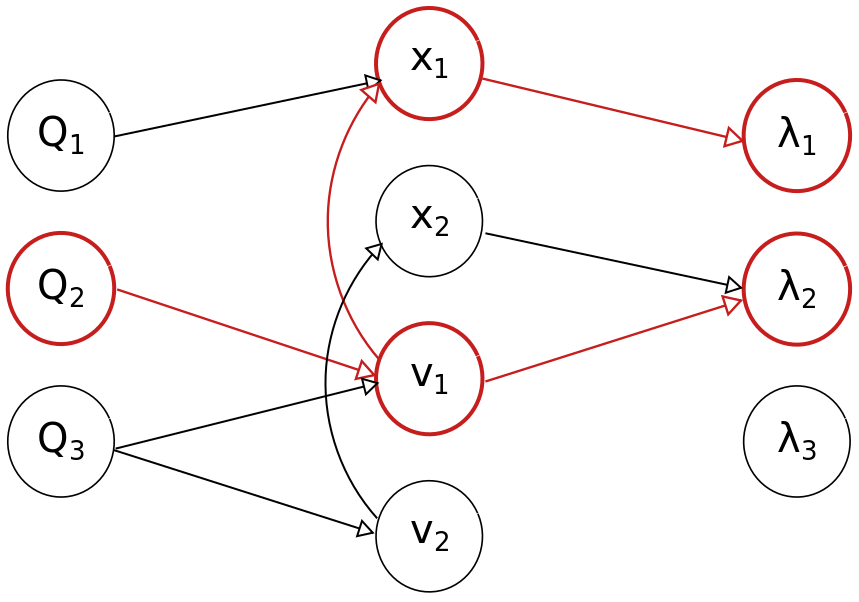
\includegraphics[width=.5\textwidth]{img/ch3-dependencies-graph}
  \caption{A graphical representation of an imaginary dependencies graph for
           a PDMP on a $4$-dimensional position-velocity state space.
           The arrows represent the dependencies between the nodes.
           The vertical arrows between the state space variables are
           induced by $\text{Dep}_{\phi}$ function (in this case
           $\phi$ is the linear flow, whose implementation is given in
           Listing~\ref{linear-flow-implementation}).
           The red nodes and edges depict the procedure
           for finding which factors need to be resimulated, after invocation
           of a specific Markov kernel (which is $\mathcal{Q}_{2}$ in this image).}
  \label{image-dependencies-graph}
\end{SCfigure}

We will now describe how to incorporate this graph into our PDMP framework.
It is indeed very easy to do: we simply instantiate the Markov kernel and the Poisson process
policies, by giving the graph via a constructor argument.
Both policies can then decide exactly what they need to take from the graph in order
to set up its state. In our implementation, the Markov kernel policy simply
takes all the Markov kernel nodes, while the Poisson process policy takes the
factor nodes and will repeatedly query the graph for the dependencies between
the Poisson processes. There are implicit assumptions that the user of the
library has to be avare of. We assume that the generator of the process is
of the form given in Equation~\ref{pdmp-generator-n-components}, so that the
number of factor and Markov kernel nodes must be the same (our implementation
perform compile-time checking of this assumption), and $i$-th factor
node corresponds to the $i$-th Markov kernel. Also, the number
of variable nodes has to be equal to the dimensionality of the process
state space.
Finally, the flow policy needs to extend its interface
to support for $\text{Dep}_{\phi}$ calculation (not shown here, see the code
repository for details). A particularly nice feature of C++ class templates
is that if a method of some template class is never called, the compiler ignores it
so that it does not even appear in the resulting binary.
So extending the flow interface does not impose any performance penalties
for PDMP simulations which do not require such functionality.

The interface of the dependencies graph is given in Listing~\ref{listing-dependencies-graph}.
There is the last design choice to consider regarding the dependencies graph.
One way to do the dependencies calculations is to look at the variables
modified by the markov Kernel at every iteration of the process and simply
find i


\begin{lstfloat}
\caption{An interface of the dependencies graph.}
\label{listing-dependencies-graph}
\begin{lstlisting}
template<
  int N, int StateSpaceDim,
  class MarkovKernelNodeType, class VariableNodeType, class FactorNodeType>
class DependenciesGraph {
 public:

  using MarkovKernelNodes = array<shared_ptr<MarkovKernelNodeType>, N>;
  using VariableNodes = array<shared_ptr<VariableNodeType>, StateSpaceDim>;
  using FactorNodes = std::array<std::shared_ptr<FactorNode_t>, N>;

  // Create the graph by simply providing the nodes.
  DependenciesGraph(
    const MarkovKernelNodes& markovKernelNodes,
    const VariableNodes& variableNodes,
    const FactorNodes& factorNodes);

  template<class Flow = LinearFlow>
  const std::vector<int>& getFactorDependencies(int factorId);

  const MarkovKernelNodes markovKernelNodes;
  const VariableNodes variableNodes;
  const FactorNodes factorNodes;
};
\end{lstlisting}
\end{lstfloat}


\begin{lstfloat}
\caption{The implementation of Markov kernel nodes.}
\label{markov-kernel-nodes-implementation}
\begin{lstlisting}
template<class State>
struct MarkovKernelNodeBase {
  ~MarkovKernelNodeBase() = default;
  virtual State jump(const State& state) = 0;
  const std::vector<int> dependentVariableIds;
};

template<class State, class JumpFunctor>
class MarkovKernelNode : public MarkovKernelNodeBase<State> {
 public:

  MarkovKernelNode(
    const std::vector<int>& dependentVariableIds,
    const JumpFunctor& jumpFunctor);

  virtual State jump(const State& state) override final {
    auto stateSubvector = state.getSubvector(this->dependentVariableIds);
    auto modifiedSubvector = this->jumpFunctor_(stateSubvector);
    return state.constructStateWithModifiedVariables(
      this->dependentVariableIds, modifiedSubvector);
  }

 private:
  JumpFunctor jumpFunctor_;
};

// The client code can then create the nodes as follows:
auto jumpKernel = [] (auto stateSubvector) -> {
  ... // Do something with stateSubvector.
  return modifiedStateSubvector;
};
MarkovKernelNodeBase* = new MarkovKernelNode<decltype(jumpKernel)>(
    {1, 2}, // Specify the variable indices on which this kernel acts.
    jumpKernel);

\end{lstlisting}
\end{lstfloat}


\begin{lstfloat}
\caption{The Poisson process policy based on the dependencies graph.}
\label{main-poisson-process-policy-implementation}
\begin{lstlisting}
template<
  class DependenciesGraph,
  template<class> class EventScheduler = PriorityQueueEventScheduler>
class PoissonProcessPolicy {
 public:

  // Provide the dependencies graph via a constructor argument.
  PoissonProcess(DependenciesGraph graph);

  // The method which will be invoked by the PDMP host class.
  template<class State, class HostClass>
  auto getJumpTime(const State& state, const HostClass& hostClass) {
    resimulateEventsForFactors(factorsToResimulate_);
    while (true) {
      Event event = eventScheduler_.pop();
      int factorId = event.factorId;
      if (!event.isValid) {
        // This event was invalidated because a new event was
        // simulated for this factorId.
        continue;
      }
      if (!event.shouldAccept()) {
        // Event was rejected due to the Poisson process thinning step.
        resimulateEventForFactor(factorId);
        continue;
      }
      // Found an event that is valid and not rejected.
      factorsToResimulate_ =
        graph_.getFactorDependencies<HostClass::FlowPolicy>(factorId);
      auto iterationTime = event.time - currentTime_;
      currentTime_ = event.time;
      return iterationTime;
    }
  }

  // This method will be accessed by the Markov kernel policy.
  int getLastFactorId() const;

 private:
  EventScheduler<Event> eventScheduler_;
  DependenciesGraph graph_;
  vector<int> factorsToResimulate_;
  double currentTime_ = 0.0f;
};
\end{lstlisting}
\end{lstfloat}


\begin{figure}
  \centering
  \def\svgwidth{.95\linewidth}
  \input{ch3-uml-diagram.pdf_tex}
  %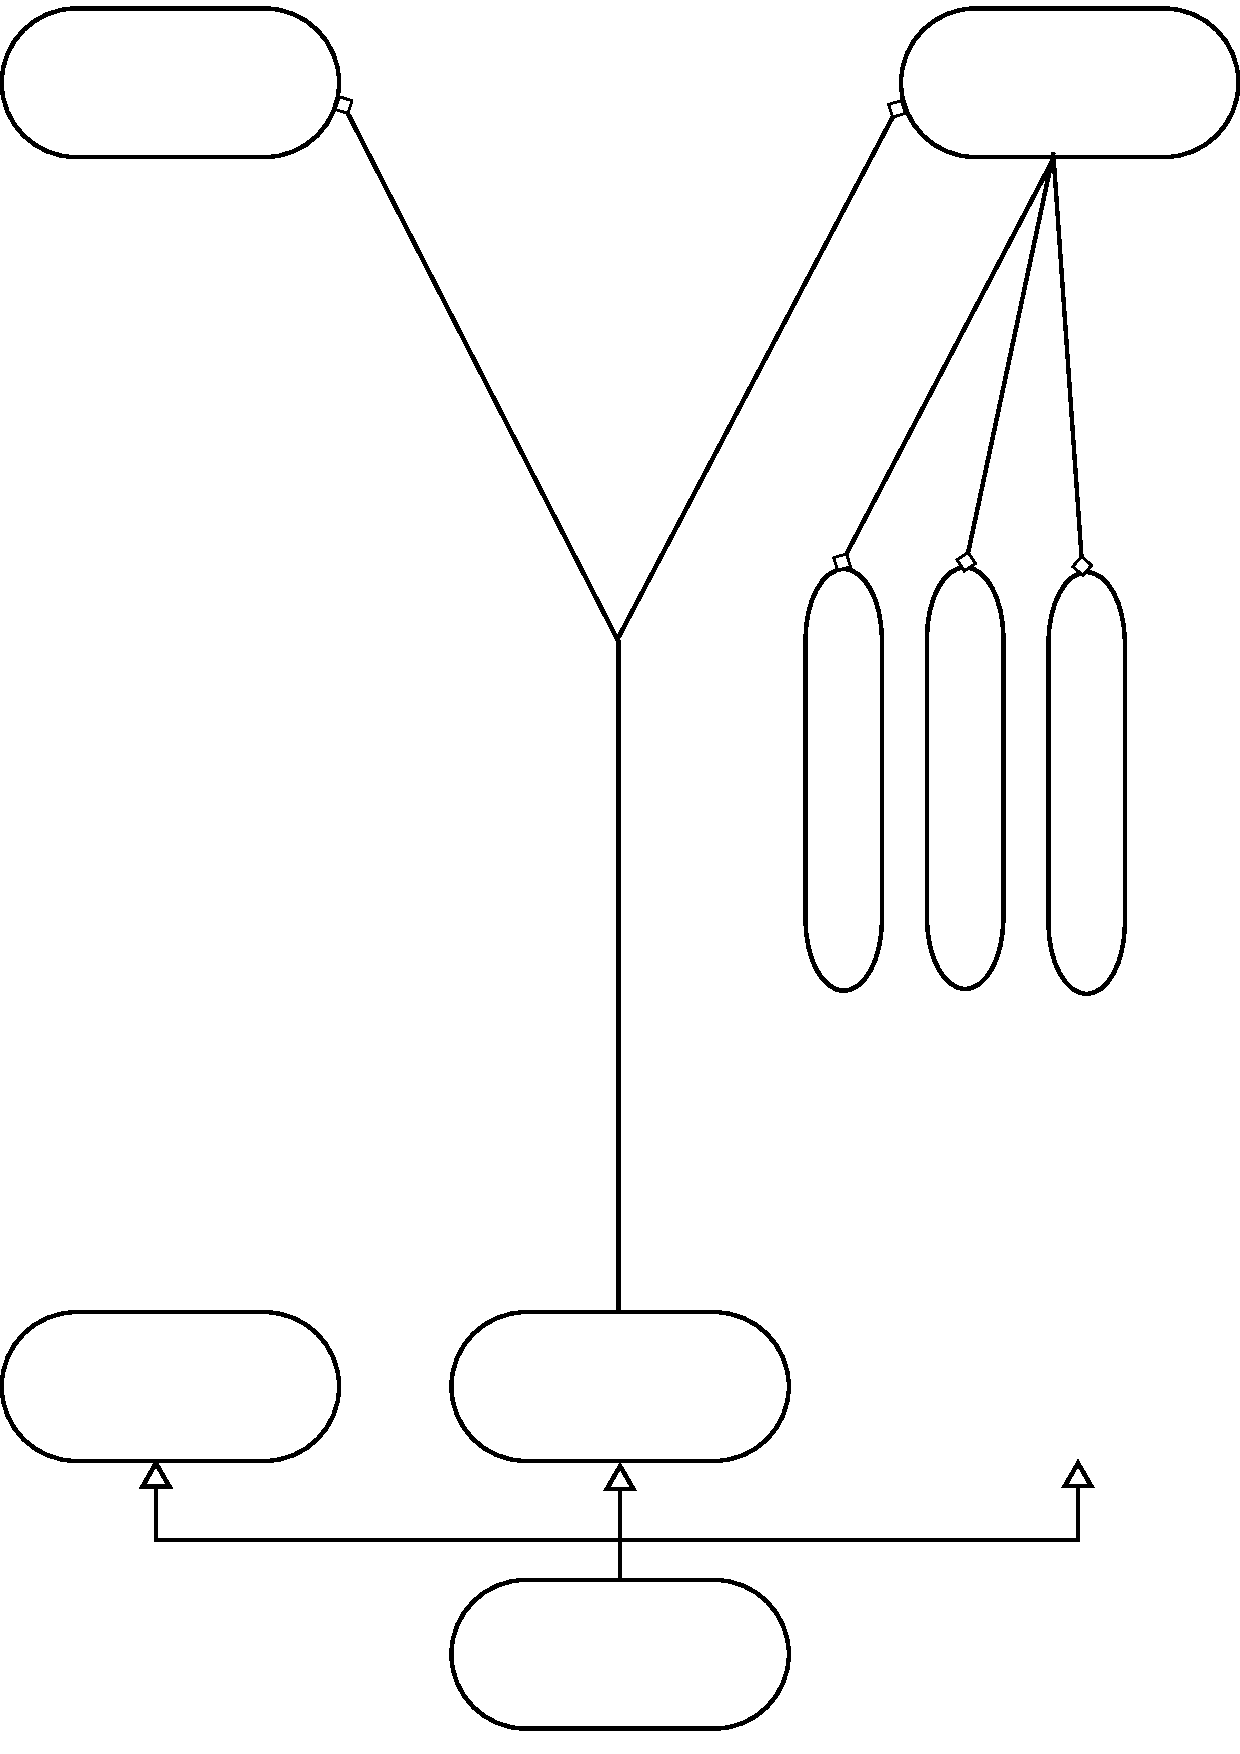
\includegraphics[width=0.9\textwidth]{img/ch3-uml-diagram}
  \caption{A UML diagram depicting the final design of our PDMPs simulation framework.
           The dashes lines represent pointers, edges ending in a white triangle
           represent inheritance, edges with a diamond shaped ending the
           has-a relationship. Red circles represent the events not yet removed
           from the events schedulerr, but who have already been invalidated.}
  \label{image-uml-diagram-dependencies-graph-based-design}
\end{figure}

Dependencies graph\\
Resolve at runtime vs caching? We choose caching, since we can always split up Markov kernels as much as we want.\\
Event scheduling (mention discrete event simulation from Levroye)\\
Rejection sampling, lambda callbacks\\
Class diagram

\section{Testing}

The importance of writing automated tests for any kind of software cannot be overstated.
As the project grows in size, small code changes can have seemingly unexpected consequences.
It becomes hard to reason about the correctness of our code and as a result,
subtle bugs get introduced to the production code, which can be especially hard to
track down later. To help alleviate these problems, we turn to unit and integration testing,
which will try to make sure, that any future changes to the code will not break the
correctness conditions.

We use Google's googletest\footnote{
See https://github.com/google/googletest.}
framework for writing tests and mocking objects.
At first we test each of the individual component discussed in this chapter, by
replacing their dependencies with mock copies, whose behaviour can be controlled precisely.
This idea is at the heart of unit testing -- we are able to test the correctness of a
specific component regardless of the correctness of its dependencies
(and the dependencies of its dependencies, for that matter).
Next, we write integration tests to see if the components behave correctly as a unit.
An interesting issue arises in our case, because we want to test an inherently random
processes. The process outcome is hence allowed to be different during different
runs, which makes testing harder.
We resolve this issue by mocking the random number generators (RNG), then performing
a short simulation by hands (using the mock RNG output, which we can set up ourselves)
and test if they match our process output.

We have tried to cover as much of the edge cases as possible by writing tests
for the PDMPs framework discussed in this section. A total of 35 test cases were
written, the source code of which can be found in tests/core directory of the
project's GitHub page.

\end{document}
